% !TEX root = ../main.tex
\section{Introduction}
\label{sec:intro}

A deployment decision is, implicitly, a bet that a benchmark rank still holds at the new site. The
bet fails for a reason that is mechanical rather than statistical: a score is an outcome measure, and
an outcome can be right for the wrong reason. A
policy that never approaches a pedestrian because it plans short trajectories scores as well as one
that sees the pedestrian and yields, and the two behave very differently the first time the scene
changes. Telling them apart means asking \emph{why} the score came out as it did, usually from little
data: a closed-loop simulator for the target domain, or a fleet
test, is exactly what the decision is meant to save.

%120
% 这被定义成从benchmark往部署域迁移的问题，目前各家的做法是进行大规模的真实部署场景的测试，然后再依据反馈进行模型调整和后训练，如此往复，造成大量的测试资源花销，同时也延长了模型迭代的周期。
We frame this as a transfer problem from the benchmark to the deployment domain. Current practice
closes the gap empirically: a candidate policy is exercised at scale in the target domain, adjusted
and post-trained on the resulting feedback, and exercised again, the loop repeating until its
behaviour is judged acceptable. Every turn of that loop consumes substantial testing resources and
lengthens the development cycle.



%120
% 目前提出了很多跨域的研究「如域自适应、域泛化等」，但多集中在点出问题，和模型的训练解决，而缺乏对策略在目标域表现的系统性评估。并不能实质解决部署时候的选型难题。
% 在论文「dont blind your vla」中，制作了think-site表征语言图像分割程度；然而，这个套件的迁移只适用于v-l多模态模型，无法横展到一些仅解码器的扩散策略评估，并且仍建立在已有被选中模型的基础上研究如何提升模型能力，也无法系统回答模型选型时该如何决策。
% 在RepE论文中，作者给出了RepE的方法来定位和修复域间gap，但该方法旨在暴漏大语言模型在语义刺激下的反馈，又难以横展到读入图片的物理AI策略的评估。
% 「再举一些LLM测迁移如function vector」的例子，说明当前在大语言模型的迁移评估上已有一定的研究，但这些方法仍难以直接应用于物理AI策略的跨域评估。物理AI策略的跨域评估仍然缺乏系统性的方法。
A considerable body of cross-domain work has been proposed---domain adaptation, domain generalisation
and the like---but it concentrates on identifying the problem and on solving it through training, and
lacks any systematic assessment of how a policy behaves in the target domain. It therefore does not
substantively address the selection problem that arises at deployment.

In \emph{Don't Blind Your VLA}~\cite{TODO-blindvla}, a think-site representation is built to measure
the degree of language--image segmentation; the transfer of that suite, however, applies only to
vision--language multi-modal models and does not extend to the evaluation of decoder-only diffusion
policies, and it is still built upon an already-chosen model, studying how that model's capability may
be improved rather than answering systematically how a model should be selected.

In the RepE paper~\cite{zou2023repe} the authors give a method for locating and repairing the gap
between domains, but it is aimed at exposing a large language model's response to semantic stimuli,
and is likewise hard to extend to the evaluation of physical-AI policies that read images.

Further work on measuring transfer in large language models, such as function
vectors~\cite{TODO-funcvec}, shows that transfer evaluation is already established there; these
methods, however, remain difficult to apply directly to the cross-domain evaluation of physical-AI
policies. A systematic method for the cross-domain evaluation of physical-AI policies is still
missing.
%120

%120
%物理AI领域该类型参考空白的结果就是，当前的自动驾驶中，很多learderboard 和开源测试集涌现，以缩小模型训练与现实部署环境之间的差距。伴随出现各种评级和榜单。如nuScenes的榜单和NAVSIM的排行榜，为研究者提供了评估策略在不同环境下表现的工具。但这些排行榜给出的表现分数多是传统的交通指标，然而当前在各大模型类方法涌现的今日，单纯的看最后结果已经无法全面反映策略的能力，往往出现榜单最优的模型在域间迁移后排名大幅下降甚至榜单失效，难以真正作为从仿真到真实部署域选型决策的依据。「加一些参考文献」
The consequence of this gap in the physical-AI literature is that the decision is left to the
leaderboards. In autonomous driving a growing number of leaderboards and open test sets have
appeared~\cite{caesar2020nuscenes,caesar2021nuplan,dauner2024navsim}, meant to narrow the gap between
the conditions a model is trained on and those it is deployed in, and with them a variety of ratings
and rankings. nuScenes' leaderboard and NAVSIM's leaderboard, for instance, give researchers a means
of assessing how a policy performs under different conditions. The scores these leaderboards report,
however, are for the most part conventional traffic metrics. With the recent proliferation of
large-model-based methods, reading the final outcome alone no longer reflects a policy's capability in
full~\cite{li2024egostatus,codevilla2019exploring,geirhos2020shortcut}.
\emph{!!!!!!!!!! ADD MORE PAPER TO REFER}
%！！！！！「加一些参考文献」%
The consequence is that a policy ranked first on a leaderboard often falls sharply once the domain changes, or the ranking
ceases to be informative at all~\cite{hendrycks2019benchmarking,xie2023robobev}, so that it cannot
serve as a sound basis for the selection decision that takes a policy from simulation into a real
deployment domain.
%120

To address this issue, we propose a \emph{check-up}:
%120
We construct pixel-level paired data and reduce each pair to two axes of causal attribution: the
\emph{faithfulness} displacement $F$, the plan change caused by the pedestrian itself, and the
\emph{interference} displacement $I$, the change the same policy produces under an edit that carries
no driving-relevant information~\eqref{eq:FI}. Reading a policy on these axes yields a prognosis for
its behaviour in the target domain: diagnosed on one driving side and tested on the other, the exam
that transfers predicts the new side's near-miss rate at $\rho={\NumSpBeh}$, whereas nuScenes'
open-loop metrics and NAVSIM's leaderboard score reach only $-0.54$--$+0.49$ against the same target;
what carries over is the ordering and the verdict. Fitting how each estimate's spread shrinks with
sample size further shows the lighting verdict settled within \NumNstarCFRhi{} frames and exposure
within \NumNstarExpHi, so a deployment decision can be priced in tens of target-domain frames rather
than in a closed-loop simulator or a fleet test. The framework therefore offers a more dependable
basis for selecting a policy for a given deployment.
%！！！！！这段增加引用文献

\begin{figure}[t]
\centering
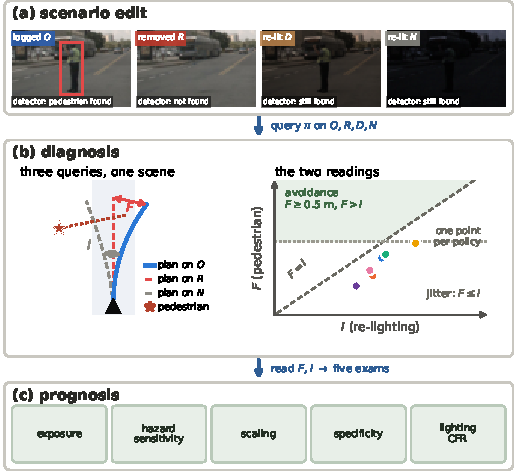
\includegraphics[width=\columnwidth]{figures/frame1c.pdf}

\caption{\textbf{check-up frame.} }
%120
% 该体检过程中，首先进行像素级配对数据的构建，然后提炼因果轴，最终对策略在目标域的表现进行预诊断。
The check-up proceeds in three stages: constructing pixel-level paired data, distilling the causal
axes from them, and issuing a prognosis for the policy's behaviour in the target domain.
\label{fig:method}
\end{figure}


% \paragraph*{Contributions}
%120
本文的贡献在于，在物理智能领域，设计了一个通用的模型体检的流程，具体包括（a）像素级配对数据的构建，（b）因果轴的提炼以及（c）prognosis:策略在这些轴上的评估的检测手段。

%120 :!!!!!!内部要改具体内容
The contribution of this paper is a general check-up procedure for physical AI, comprising 
\begin{enumerate}\itemsep2pt
\item the construction of \emph{pixel-level paired data}: built a small-sample check-up for driving policies on verified, pixel-level counterfactual
      edits of real frames rather than the promptable text prompts language-model interpretability
      usually relies on --- to our knowledge among the first uses of concept-vector-style methods on
      a multi-modal, largely non-promptable input. Its central result is methodological: raw response
      magnitude is a poor safety signal, and decomposing it into magnitude, jitter and separation turns
      a two-sided quantity into a one-sided certificate. We use it to diagnose six policies, with an
      explanation from inside the networks.


\item using the distillation of the \emph{causal axes} to diagnose: in a new domain, for the linear representation hypothesis: the faithfulness direction $\hat v_F$ (response to the pedestrian) and the interference direction $\hat v_I$ (response to a
      change with no driving-relevant information) are geometrically opposed in aggregate (mean cosine $-0.54$ across
      four policies), and this opposition is mirrored behaviourally, not just in the representation.
      The relationship is a property of the pooled data, not a stable per-policy trait
      (\cref{sec:lighting}), and we report it as such.


\item the \emph{prognosis}: an account of what small data can and cannot establish: sample-size laws for every exam and a
      pre-registered left- to right-hand-drive transfer test. The exam that transfers predicts
      behaviour on the new side better than that side's own leaderboard score does.

\end{enumerate}


% \item A small-sample check-up for driving policies, built on verified, pixel-level counterfactual
%       edits of real frames rather than the promptable text prompts language-model interpretability
%       usually relies on --- to our knowledge among the first uses of concept-vector-style methods on
%       a multi-modal, largely non-promptable input. Its central result is methodological: raw response
%       magnitude is a poor safety signal, and decomposing it into magnitude, jitter and separation turns
%       a two-sided quantity into a one-sided certificate. We use it to diagnose six policies, with an
%       explanation from inside the networks.
% \item Evidence, in a new domain, for the linear representation hypothesis: the faithfulness direction
%       $\hat v_F$ (response to the pedestrian) and the interference direction $\hat v_I$ (response to a
%       change with no driving-relevant information) are geometrically opposed in aggregate (mean cosine $-0.54$ across
%       four policies), and this opposition is mirrored behaviourally, not just in the representation.
%       The relationship is a property of the pooled data, not a stable per-policy trait
%       (\cref{sec:lighting}), and we report it as such.
% \item An account of what small data can and cannot establish: sample-size laws for every exam and a
%       pre-registered left- to right-hand-drive transfer test. The exam that transfers predicts
%       behaviour on the new side better than that side's own leaderboard score does.





% \paragraph{Displacement is not avoidance}
% What an edit yields most directly---how far the plan moves when the pedestrian is removed---is a poor
% safety signal on its own, and treating it as one inverts the ranking. We decompose it into the
% magnitude of the response, the displacement the same policy produces under an edit unrelated to the
% pedestrian (its own jitter floor), and the separation the response actually buys. On \NumSGscenes{} NAVSIM Singapore near-pedestrian scenes,
% the pedestrian
% outweighs the irrelevant edit in only \NumFgtIlo--\NumFgtIhi\% of scenes; among the cells where the
% plan did move, \NumMoveFar{} moved away from the pedestrian and \NumMoveNear{} moved towards it. The
% asymmetry that survives is one-directional and useful: a near-zero response certifies that the
% pedestrian did not enter the decision (\NumPFbig\% of scenes), while a large response certifies
% nothing.

% \paragraph{The diagnosis}
% Applied to six end-to-end policies, the check-up separates quantities a benchmark score merges
% (\cref{tab:report}). Exposure varies \NumExpLo--\NumExpHi{}$\times$ across policies, and in five of six
% the safety benefit of seeing the pedestrian does not grow with the hazard, so collisions follow how
% far a policy plans to drive rather than what it perceives. A night rendering moves every policy more
% than the pedestrian does, along the interference direction $\hat v_I$, which opposes the faithfulness
% direction $\hat v_F$ governing the pedestrian response (\cref{sec:lighting}); \cref{sec:diagnosis}
% traces the cause inside the networks.

% \paragraph{The prognosis}
% A check-up is only useful if it generalises: it must be cheap, and what it finds in one domain must
% still hold in another. We price each verdict against sample size --- most settle within a few dozen
% frames, hazard sensitivity within hundreds --- then test generality directly, pre-registering seven
% predictions from a diagnosis on 88 Boston frames and checking them after the switch to right-hand
% drive. Orderings transfer ($\rho=0.90$ against a pre-registered bar of $0.6$); point values do not
% (\cref{tab:prereg}), so we report rankings and verdicts rather than calibrated numbers. Re-measured on
% the new side, the exam that predicts behaviour there is not the one measuring how strongly a policy
% reacts but how steadily it drives ($\rho={\NumSpBeh}$ for specificity), beating the leaderboard score
% computed on that side's own scenes (\cref{sec:bench}). The bet named above is therefore answerable:
% not by trusting a leaderboard rank, but by running a check-up whose predictive exams generalise and
% are known in advance.
